To evaluate the optimization result, we benchmark the implementation on a 64 bit Arch Linux machine with a 3GHz Intel Skylake CPU i7-6600U. The throughput of 64 bit multiplication (mul, mulx) is 1 op/cycle, and throughput of 64 bit addition with carry (adc, adcx, adox) is 1 op/cycle. The peak performance is therefore 2 ops/cycle (6 Gops/s) on 1 core. GCC 6.1.1 is used with compile flags \texttt{-O3 -mavx2 -mbmi2 -madx}. 

Based on the recommended Elliptic curve parameters from the guidance standard \cite{Brown:2010}, we have chosen five predefined curves with various key sizes: 192, 224, 256, 384, 521 bits. All versions of the implementation have been validated by using Google Test and by checking the ECDH key exchange results. In the end we compare our implementation with OpenSSL \cite{openssl}, a well known open source library, to check our implementation effect. We linked our program to a locally compiled version of OpenSSL . 

\begin{figure}[h!]\centering
  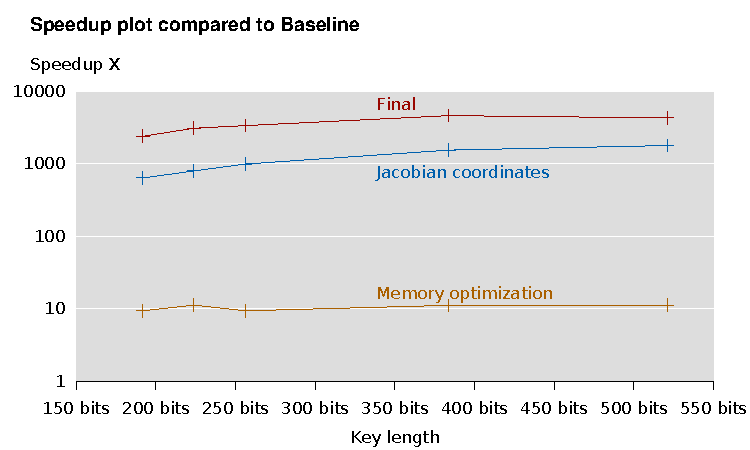
\includegraphics[scale=0.7]{speedup}
  \caption{Speedup plot compared to Baseline \label{speedup}}
\end{figure}
\begin{figure}[h!]\centering
  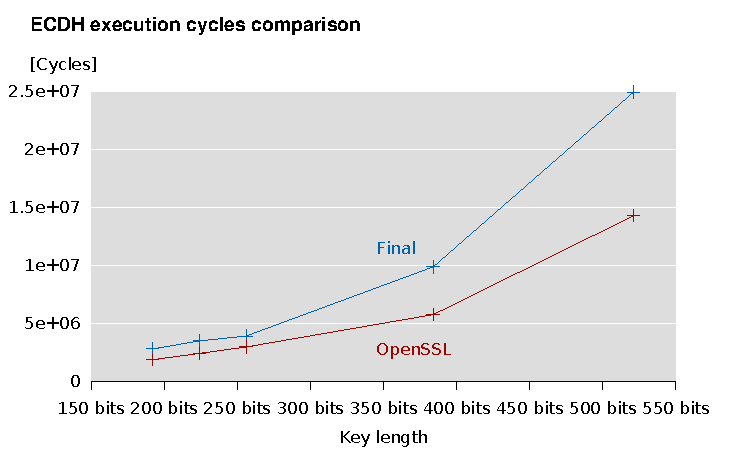
\includegraphics[scale=0.7]{ecdh}
  \caption{ECDH execution cycles comparison\label{ecdh}}
\end{figure}
\begin{figure}[h!]\centering
  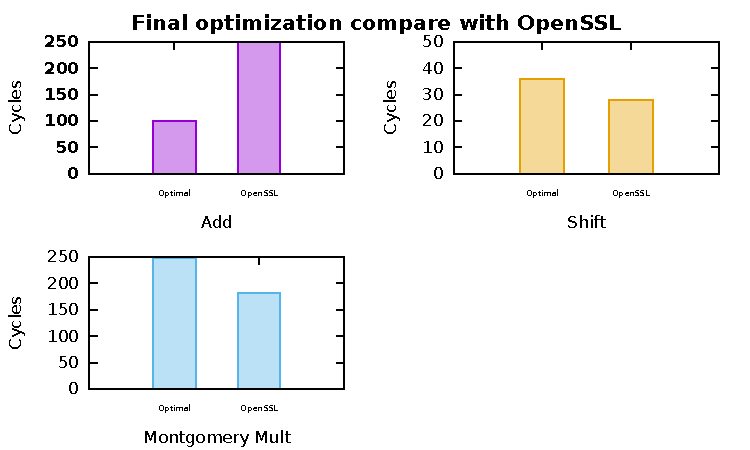
\includegraphics[scale=0.5]{openssl}
  \caption{Final optimization compared with OpenSSL\label{openssl}}
\end{figure}

In the speedup comparison (Fig.~\ref{speedup}) three crucial numbers are shown. It can be clearly seen that the Final implementation can execute the key exchange process 8900x faster than the baseline with the longest keys. The first milestone of memory optimization gives us about 10x speedup on average, whereas the Jacobian coordinates version of the code can run 1100x faster on average. This confirms the importance of the algorithmic changes explained in section \ref{sec:yourmethod}, including switching from projective to Jacobian coordinates. The resulting speedup is satisfactory and reasonable, as the first two versions of the implementation uses an inefficient memory management and a slower algorithm. The real performance boost is between the Jacobian coordinates and the Final version, after applying the architecture-specific optimizations mentioned in section 3. This gives us another 6x speedup on average, showing the efficiency of the final implementation.

Next we run the same operation using the OpenSSL library and compare the computation cycles (Fig.~\ref{ecdh}). Our number of required cycles remains the same level with OpenSSL, in key length range of less than 256 bits, yet falls behind OpenSSL with larger key length. Individual operations of integers are the main component of our algorithm. To see how good our implementation is we choose Montgomery multiplication to compare with OpenSSL (Fig.~\ref{openssl}). This comparison is done with the same input for both Final implementation and OpenSSL. Our implementation runs slightly behind OpenSSL. 

\begin{figure}[h!]\centering
  \includegraphics[scale=0.7]{perfplot1}
  \caption{Performance plot of baseline and memory optimization\label{perfplot1}}
\end{figure}
\begin{figure}[h!]\centering
  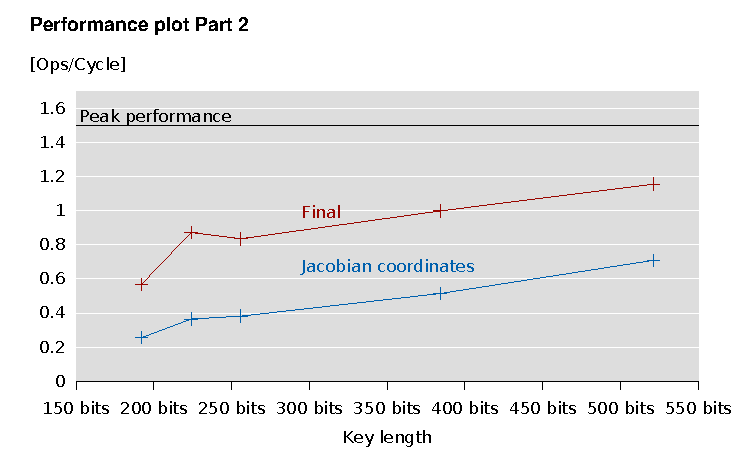
\includegraphics[scale=0.7]{perfplot2}
  \caption{Performance plot of Final optimization and Jacobian coordinates\label{perfplot2}}
\end{figure}

Performance plots (Fig.~\ref{perfplot1} and Fig.~\ref{perfplot2}) reflect if the implementation can make full use of the machines' computation ability. In Fig.~\ref{perfplot1} the first comparison is done by showing the effect of memory optimization. It is clear that with the bad memory management, the baseline performance is limited. The first approach of Memory optimization gives an increase of 4.17x in the largest key length and 4.1x in the smallest key length. In Fig.~\ref{perfplot2} we begin to see the real performance boost that comes from later optimization. Between these two figures the operation counts change drastically, thus we separate the performance plots. The peak performance here is calculated by considering the ratio of additions and multiplications. Considering the instruction balance in the main operation (Montgomery multiplication, 2 add : 1 mul), we can set the peak performance at 1.5 ops/cycle. As one can see, the final optimization are close to the peak performance with large key sizes. The highest performance of the final implementation is reached with $521$bit keys, with 1.41/1.5 = 94\% of the peak performance. From the Jacobian coordinates version to the Final we have a performance increase of 2.1x in the largest key length and 2.56x in the smallest key length. In all cases the performance increases as the key size grows. Relatively short key sizes, the setup time of the functions is relatively high compared to the time spent in the calculation loops. This prevents the program from reaching the peak performance. With longer keys the loops take most of the computation, bringing the program nearer to the peak performance.
\begin{figure}[h!]\centering
  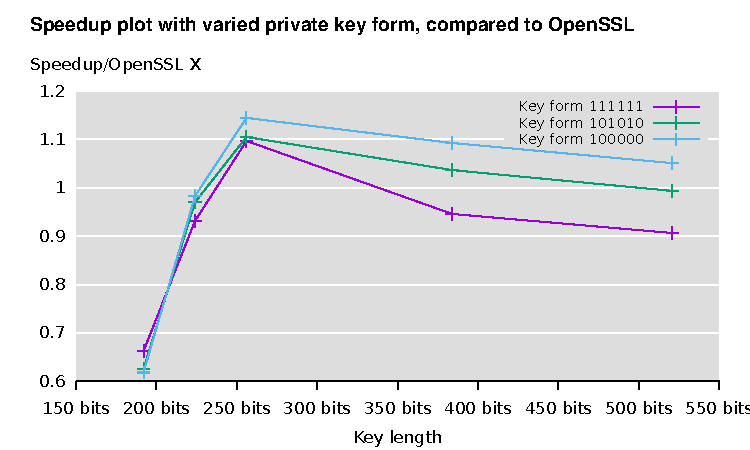
\includegraphics[scale=0.7]{keysize}
  \caption{Speedup plot with varied private key form, compared to OpenSSL\label{keysize}}
\end{figure}

Fig.~\ref{keysize} shows the our speedup compared with OpenSSL, depending on the form of the key. A key of the form 0b10..0 is optimal for the double-and-add method, since only one point addition has to be performed. Contrary to the form 0b11..1, which is the worst case scenario (see Listing \ref{lst:double_and_add}, lines 7,8). That can explain why in form 0b10..0 we are faster than OpenSSL and in form 0b11..1 we are slower. The runtime of OpenSSL seems to be independent of the key form. We assume this is a security measure for preventing side-channel attacks. So this has to be taken into consideration, when comparing the implementations.